\documentclass[useAMS,usenatbib]{mn2e}
\usepackage{graphicx}
\usepackage{hyperref}
\usepackage{tikz}
\usetikzlibrary{calc,fadings,decorations.pathreplacing}
%\usepackage{url}
\newcommand{\aj}{Astron. J.}
\newcommand{\apj}{Astrophys. J.}
\newcommand{\apjs}{Astrophys. J. Supp.}
\newcommand{\pasp}{Publ. Ast. Soc. Pac.}
\newcommand{\pasa}{Publ. Ast. Soc. Aust.}
\newcommand{\ao}{Appl. Opt.}


\newcommand\pgfmathsinandcos[3]{%
  \pgfmathsetmacro#1{sin(#3)}%
  \pgfmathsetmacro#2{cos(#3)}%
}
\newcommand\LongitudePlane[3][current plane]{%
  \pgfmathsinandcos\sinEl\cosEl{#2} % elevation
  \pgfmathsinandcos\sint\cost{#3} % azimuth
  \tikzset{#1/.style={cm={\cost,\sint*\sinEl,0,\cosEl,(0,0)}}}
}
\newcommand\LatitudePlane[3][current plane]{%
  \pgfmathsinandcos\sinEl\cosEl{#2} % elevation
  \pgfmathsinandcos\sint\cost{#3} % latitude
  \pgfmathsetmacro\yshift{\cosEl*\sint}
  \tikzset{#1/.style={cm={\cost,0,0,\cost*\sinEl,(0,\yshift)}}} %
}
\newcommand\DrawLongitudeCircle[2][1]{
  \LongitudePlane{\angEl}{#2}
  \tikzset{current plane/.prefix style={scale=#1}}
   % angle of "visibility"
  \pgfmathsetmacro\angVis{atan(sin(#2)*cos(\angEl)/sin(\angEl))} %
  \draw[current plane] (\angVis:1) arc (\angVis:\angVis+180:1);
  \draw[current plane,dashed] (\angVis-180:1) arc (\angVis-180:\angVis:1);
}

\newcommand\DrawHalfLongitudeCircle[2][1]{
  \LongitudePlane{\angEl}{#2}
  \tikzset{current plane/.prefix style={scale=#1}}
   % angle of "visibility"
  \pgfmathsetmacro\angVis{atan(sin(#2)*cos(\angEl)/sin(\angEl))} %
  \draw[current plane] (\angVis:1) arc (\angVis:\angVis+90:1);
%  \draw[current plane,dashed] (\angVis:1) arc (\angVis-90:\angVis:1);
}
\newcommand\DrawLatitudeCircle[2][1]{
  \LatitudePlane{\angEl}{#2}
  \tikzset{current plane/.prefix style={scale=#1}}
  \pgfmathsetmacro\sinVis{sin(#2)/cos(#2)*sin(\angEl)/cos(\angEl)}
  % angle of "visibility"
  \pgfmathsetmacro\angVis{asin(min(1,max(\sinVis,-1)))}
  \draw[current plane] (\angVis:1) arc (\angVis:-\angVis-180:1);
  \draw[current plane,dashed] (180-\angVis:1) arc (180-\angVis:\angVis:1);
}

%% document-wide tikz options and styles

\tikzset{%
  >=latex, % option for nice arrows
  inner sep=0pt,%
  outer sep=2pt,%
  mark coordinate/.style={inner sep=0pt,outer sep=0pt,minimum size=3pt,
    fill=black,circle}%
}

\title[FermiFAST]{FermiFAST: A Fast Algorithm for Finding Point Sources
in the Fermi Data Stream}
\author[A. Ashathaman, A. Barton and J. S. Heyl]{Asha Ashathaman$^{1}$, Alistair Barton,
  Jeremy S. Heyl$^{1}$\thanks{Email: heyl@phas.ubc.ca; Canada Research Chair} \\
$^{1}$Department of Physics and Astronomy, University of British
Columbia, 6224 Agricultural Road, Vancouver, BC V6T 1Z1, Canada}


\begin{document}
\date{Accepted ---. Received ---; in original form ---}

\pagerange{\pageref{firstpage}--\pageref{lastpage}} \pubyear{2015}

\maketitle

\label{firstpage}

\begin{abstract}
  This paper presents a new and efficient algorithm for finding point
  sources in the photon event data stream from the Fermi Gamma-Ray
  Space Telescope.  It can rapidly construct about most significant
  half of the Fermi Third Point Source catalogue (3PSC) with greater
  than 80\% purity from the four years of data used to construct the
  catalogue.  If a higher purity sample is desirable, one can achieve
  a sample that includes the upper quartile of Fermi 3PSC with only
  five percent of the sources unassociated with Fermi sources.
  Outside the galaxy plane, the contamination is essentially
  negligible.  This software allows for rapid exploration of the Fermi
  data, simulation of the source detection to calculate the selection
  function of various sources and the errors in the obtained parameters
  of the sources detected.
\end{abstract}

\begin{keywords}
methods: data analysis --- methods: observational --- techniques:
image processing --- astrometry
\end{keywords}

\section{Introduction}

{\bf more to add here and references everywhere }

\section{The Photon Database}

The key to the speed of this algorithm is the database that contains
the position of the observed photons on the sky.  Each photon is
stored in a four-dimensional $k-d$~tree
\citep{Bentley:1975:MBS:361002.361007}.  We use the particularly
memory efficient implementation of \citet{LangPhD} (used in
astrometry.net).  The coordinates are actually stored as shorts
instead of floats to save additional memory.  The typical coordinates
range from $-1$ to $+1$, so using shorts yields an angular precision
of about six arcseconds much finer than that of the Fermi point-spread
function (PSF).  This memory efficient implementation allows us to
store all of the photons detected by Fermi above 100~MeV and within a
zenith angle of 100 degrees in memory simulataneously.

The first three dimensions contain the position of the photon on the
celestial sphere as shown in the upper portion of
Fig.~\ref{fig:sphere}.  Storing the direction of the photon momentum
in this manner removes the coordinate singularity of the spherical
coordinates.  Additionally it makes integrating over the celestial
sphere straightforward because $\int d\Omega = \int 2\pi \delta p d
\delta p$ where $\delta {\bf p} = {\bf p}' - {\bf p}$ is the three
dimensional vector between two points on the sphere.  The fourth
coordinate that we denote by $w$ depends on the point-spread function
for the photon in question.  In particular $w=\pm
\sqrt{R^2_\mathrm{max}-R_i^2}$ where $R_i$ is the radius of the
ninety-fifth percentile at the energy, entrance angle and front or
back conversion for the photon.  For convenience we use positive
values of $w$ for front-converted photons and negative values of $w$
for back-converted photons.  Furthermore, $R_\mathrm{max}$ is the
ninety-fifth percentile for the photon with the poorest angular
resolution.  This is depicted in the lower panel of
Fig.~\ref{fig:sphere}.
\begin{figure}
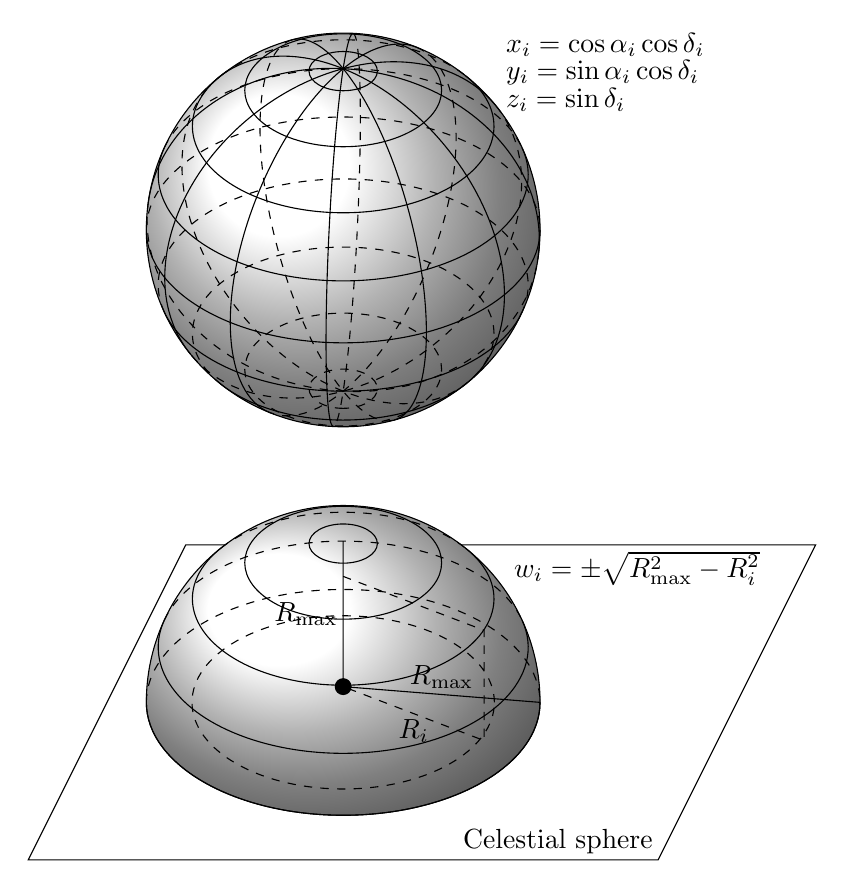
\begin{tikzpicture} % "THE GLOBE" showcase

\def\R{2.5} % sphere radius
\def\angEl{35} % elevation angle
\filldraw[ball color=white] (0,0) circle (\R);
\foreach \t in {-80,-60,...,80} { \DrawLatitudeCircle[\R]{\t} }
\foreach \t in {-5,-35,...,-175} { \DrawLongitudeCircle[\R]{\t} }
\draw (2,2.35) node [right] {$x_i=\cos\alpha_i\cos\delta_i$} 
      (2,2.0) node [right] {$y_i=\sin\alpha_i\cos\delta_i$}
      (2,1.65) node [right] {$z_i=\sin\delta_i$};
\begin{scope}[shift={(0,-6)}]
\draw (-4,-2) -- (-2,2) -- (6,2) -- (4,-2) -- cycle;
\draw (4,-2) node [above left] {Celestial sphere};
\filldraw[ball color=white] (0:\R) arc (0:180:\R)
(0,0) (0:\R) arc (0:-180:2.5 and 1.433904196);
\foreach \t in {0,20,...,80} { \DrawLatitudeCircle[\R]{\t} }
\draw (2.1,1.7) node [right] {$w_i=\pm\sqrt{R^2_\mathrm{max}-R^2_i}$};
\draw (0,0.2) -- node [above] {$R_\mathrm{max}$} (\R,0)
      (0,0.2) -- node [left] {$R_\mathrm{max}$} (0,0.81916*\R);
\draw [dashed] (0,1.6) -- ++(1.79,-0.6855) -- ++(0,-1.4) 
      -- node [below] {$R_i$} (0,0.2)
      (0,0.0) circle (1.92 and 1.10);
\filldraw[black] (0,0.2) circle (0.1);
\end{scope}
\end{tikzpicture}
\caption{The location of a given photon event on the celestial sphere
  and in the additional dimension. $R_i$ is the ninety-fifth
  percentile radius for the photon in question and $R_\mathrm{max}$ is
  the largest ninety-fifth percentile radius for the photons in the
  sample.}
\label{fig:sphere}
\end{figure}

Once the $k-d$~tree is created, it is efficient to find all of the
entries within the database within a given Cartesian distance of a
particular point.  In our case we query the database for all of the
photons within a distance $R_\mathrm{max}$ of a particular point on
the celestial sphere and use $w=0$ for the fourth coordinate.  The
particular choice of $w$ for the observed photons means that the query
will yield all of the photons that are within the ninety-fifth
percentile of the PSF.  In other words, if there is a point source
located at that particular point the query will return on average 95\%
of the photons from that source.  Of course, it will also return
photons from the background and other nearby sources.  This means that
the region of interest for a particular prospective source is energy
dependent.  The form of the exposure map also is energy dependent as
shown in Fig.~\ref{fig:expmap}.  It peaks at 0.95 times the exposure
time in the direction of the potential source and slowly drops to the
ninety-fifth percentile of the PSF in radius and then drops according
to the power-law of the tail component of the linear combinations of
King function that are used to characterize the Fermi PSF. 
\begin{figure}
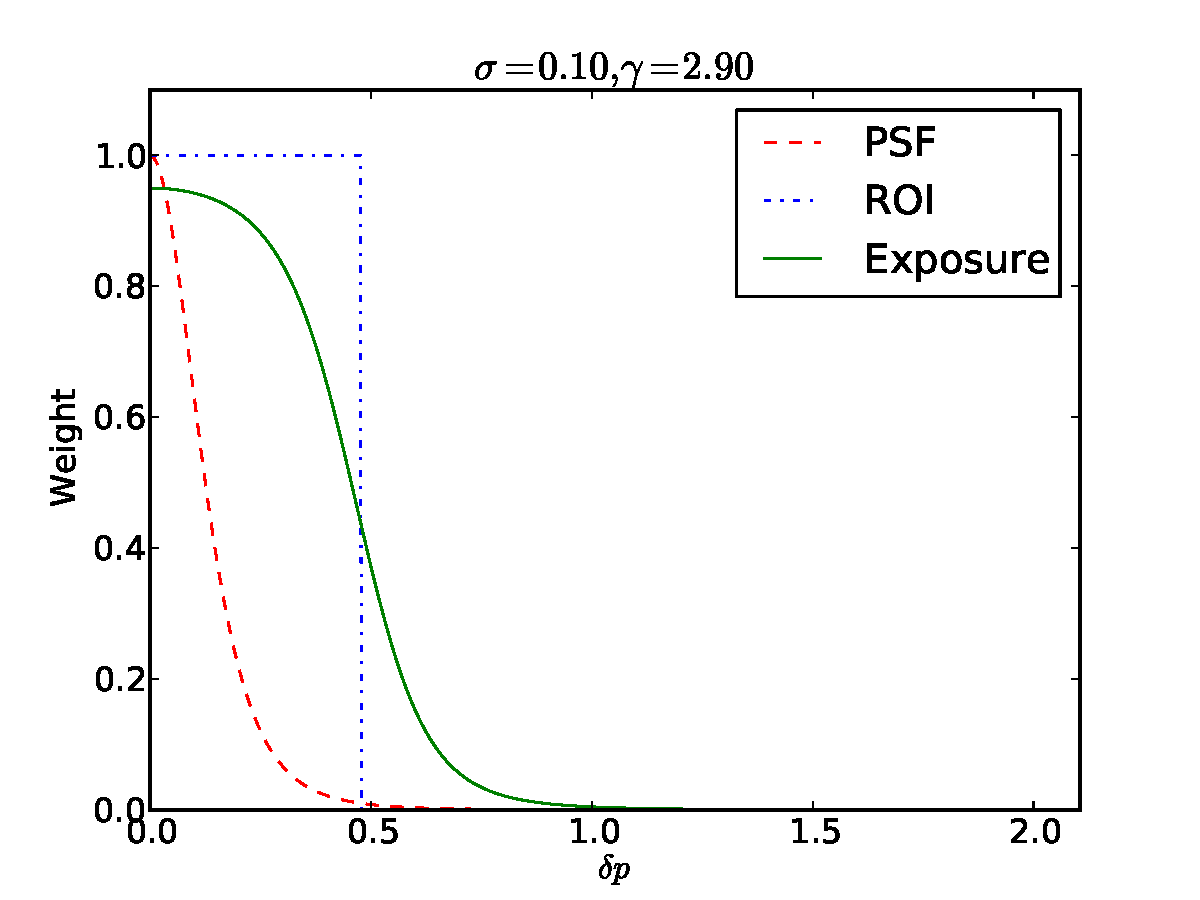
\includegraphics[width=\columnwidth]{expmap}
\caption{The Exposure Map, Region of Interest (ROI)
  and Point-Spread Function (PSF)}
\label{fig:expmap}
\end{figure}

Altough the construction of the tree is not done in parallel, the
queries are performed in parallel using the tree held in shared
memory.  For example if one uses all the photons above 100~MeV from
weeks 9 through 216 with a standard zenith angle cut of less than 100
degrees (89,684,009 photons) requires one gigabyte to store the tree
and about ten minutes to construct. The 200,000 location queries and
likelihood calculations require 140,000 seconds (700~ms each), so the
speed-up through parallisation can be dramatic.  On the other hand, if
one restricts to photons above 1~GeV (13,193,171), it only takes 90
seconds to construct the tree.  At higher energies, it makes sense to
make more location queries because the PSF is smaller.  In this
example 786,426 queries require 5,600 seconds of CPU time (7~ms each)
or only six minutes on sixteen cores.

\section{Source Likelihood}

Using the $k-d$~tree to determine the photons that would like within
the 95\% enclosure region of the point-spread function, we calculate
several statistics of the observed photons to assess the likelihood of
a source being at a particular position on the sky.  We first
determine two statistics whose distributions are known. First, if all
of the photons within the region of interest (all photons that lie
within the 95th-percentile cone of the potential source) indeed come
from a uniform background, the ratio of the solid angle enclosed in a
circle centred on the potential source and running through the
observed to the total solid angle within the region of interest for
that particular photon should be uniformly distributed between zero
and one.  We denote the mean of this ratio over the observed photons
$\bar r^2$.  This is a Bates distribution with mean of $1/2$ and
variance of $1/(12 N_\mathrm{photons})$.  Second, if all of the photons within the
region of interest indeed come from a point source at the centre of
the region of interest, the ratio of the percentile of a given photon
within the cumulative PSF distribution for that particular photon to
0.95 should be uniformly distributed between zero and one.  We denote
this statistic by $\bar f$.

If we assume that the observed photons originate from a linear
combination of these two possiblities, we can determine the ratio of
the two contributions from these statistics. In particular the fraction
of photons that come from the point source would be
\begin{equation}
  A_f=\frac{\frac{1}{2}-\bar r^2}{\bar f-\bar r^2}
  \label{eq:1}
\end{equation}
and we can estimate the significance of the value of $A_f$ by
\begin{equation}
  S(r^2) = \left ( \bar r^2-\frac{1}{2} \right ) \sqrt{12 N_\mathrm{photons}}
\label{eq:2}
\end{equation}
and the probabilty of getting a value of $S(r^2)$ larger than $x$ by
chance is
\begin{equation}
  P\left [ S(r^2) > x \right ] = \frac{1}{2} \mathrm{erfc} \left ( \frac{x}{\sqrt{2}} \right
  ) \approx \exp \left (-\frac{x^2}{2} \right )
  \label{eq:3}
\end{equation}
if we take the limit of many photons in the region of interest where
the Bates distribution tends to the normal distribution.  

\begin{table*}
  \caption{Basic statistics calculated for the photon distribution around a potential source}
  \label{tab:stats}
  \begin{tabular}{l|cll}
    \hline
    Statistic & Symbol & Abbreviation & Definition \\
    \hline
    Number of photons                     &  $N_\mathrm{photons}$ & \texttt{N}        & Number of photons that lie within the 95\% percentile \\
    Mean Solid Angle Ratio                &  $\bar r^2$          & \texttt{MEANR2}   & The mean of the ratio of solid angle enclosed between observed \\
                                          &                      &                   & photon position and source location and the solid angle \\
                                          &                      &                   & enclosed with the 95\% percentile of the PSF \\
    Mean Percentile Ratio                 &  $\bar f$            & \texttt{MEANFRAC} & The mean of the ratio of PSF percentile to 95\% \\
    Significance of \texttt{MEANR2}       & $S(r^2)$             & \texttt{SIGR2}    & How many standard deviations is \texttt{MEANR2} away from 0.5 \\
    Significance of \texttt{MEANFRAC}     & $S(f)$               & \texttt{SIGFRAC}  & How many standard deviations is \texttt{MEANFRAC} away from 0.5 \\
    Fraction of photons from point source & $A_f$                & \texttt{AFRAC}    & If one assumes that the photons come from the sum of a  \\
                                          &                      &                   & uniform background and a point source, what fraction \\
                                          &                      &                   & come from the point source? $A_f=(0.5-\bar r^2)/(\bar f-\bar r^2)$ \\
%    Mean Solid Angle Ratio of Model       & \texttt{BVAL}        &                  & What is the expected mean solid angle ratio given the model \\
%                                          &                      &                  & using \texttt{AFRAC} above? $\mathtt{BVAL}=\mathtt{SUMR2}-\mathtt{SUMFRAC}+0.5$
  \end{tabular}
\end{table*}

These basic statistics are summarized in Tab.~\ref{tab:stats}, and
Tab.~\ref{tab:topten} lists these statistics for the ten most
significant sources detected.  These basic statistics really just
compare two numbers about the distribution of the photons within the
region of interest.  We can use the detailed knowledge of the point
spread function to develop a more comprehensive test of the
distribution of photons.  In particular we define the unbinned
likelihood
\begin{equation}
  \log L = \sum_\mathrm{photons} \log \left [ A_\mathrm{PSF} \frac{\mathrm{PSF}_i \Omega_{\mathrm{max},i} }{0.95} + (1
    - A_\mathrm{PSF}) \right ]
  \label{eq:4}
\end{equation}
where we have dropped $N_\mathrm{pred}$ from the usual definition
because we have defined the model in such a way that
$N_\mathrm{pred}=N_\mathrm{photons}$ automatically and
$d N_\mathrm{pred}/dA_\mathrm{PSF}=0$.  Furthermore, for
$A_\mathrm{PSF}=0$, $\log L=0$ and because we are fitting a single
variable, $\log L$ is distributed as a chi-squared distribution with a
single degree of freedom and the probability of getting a value
of $\log L$ larger than $x$ by chance is
\begin{equation}
  P(\log L > x) = \sqrt{\pi} \mathrm{erfc} \left ( \sqrt{\frac{x}{2}}
  \right ) \approx \exp \left (-\frac{x}{2} \right ).
  \label{eq:5}
\end{equation}
From Tab.~\ref{tab:topten} we can see that the values of $A_f$ are
similar to those of $A_\mathrm{PSF}$ at least for highly significant
sources.

The first pass is to determine the value of $\log L$ on a HEALPix grid
of potential sources.  For example for the photons above 1~GeV we used
$\mathtt{NSIDE}=256$ or 786,432 grid points.  Of these 786,432 points,
18,425 have $P(\log L >x) < e^{-12.5} \approx 4 \times 10^{-6}$.  Next
we take this list of potentially significant sources and find the
local maxima of $\log L$; this reduces the number to 1,226 unique
potential sources.  However, 426 have $A_\mathrm{PSF}<0$, indicating
not a source but a point-like deficit, leaving 800 sources.  Each of
these potential source positions is used more precisely to determine
the local maxima of $\log L$ and get a more precise position for each
source.  For the lower-energy cutoff, we start with
$\mathtt{NSIDE}=128$ or 196,608 grid points.  Of these 196,608 points,
96,066 have $P(\log L >x) < e^{-12.5} \approx 4 \times 10^{-6}$
and 967 unique peaks of which 310 have $A_\mathrm{PSF}>0$.

Before discussing the results ({\em i.e.} the catalogue of sources and
how they compare with the third Fermi catalogue, we will examine the
performance of the technique and focus on the sources detected from
photons with energies exceeding 1~GeV.  The left-panel of
Fig.~\ref{fig:acorr} depicts the results of the initial set of peaks
with $P(\log L)<e^{-12.5}$ before position refinement.  We see that
for $A_f>0$ there is a strong linear correlation between the value of
$A_f$ and $A_\mathrm{PSF}$.  Whereas for negative values of $A_f$
where there is a hole in the photon distribution, the value of
$A_\mathrm{PSF}$ saturates at $-0.1$. The right panel shows the values
of $A_\mathrm{PSF}$ against the significance.  There are both
significant sources and holes in the photon distribution.  The
fractional deficit in the ``hole'' regions is limited to one tenth.
Because of the focus of this paper is to look for gamma-ray sources,
we won't discuss these ``holes'' further, but they would be an
interesting focus of further investigation. 
\begin{figure*}
  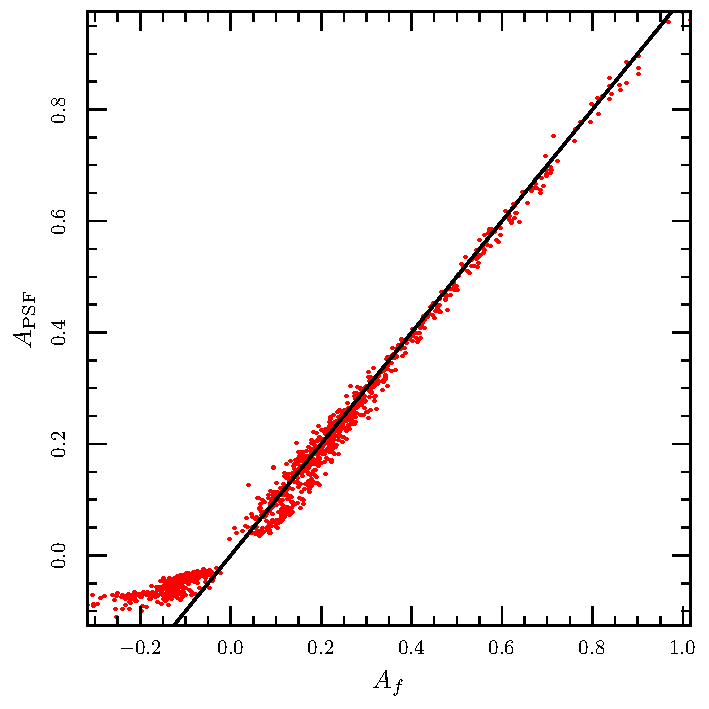
\includegraphics[width=\columnwidth]{acorr}
  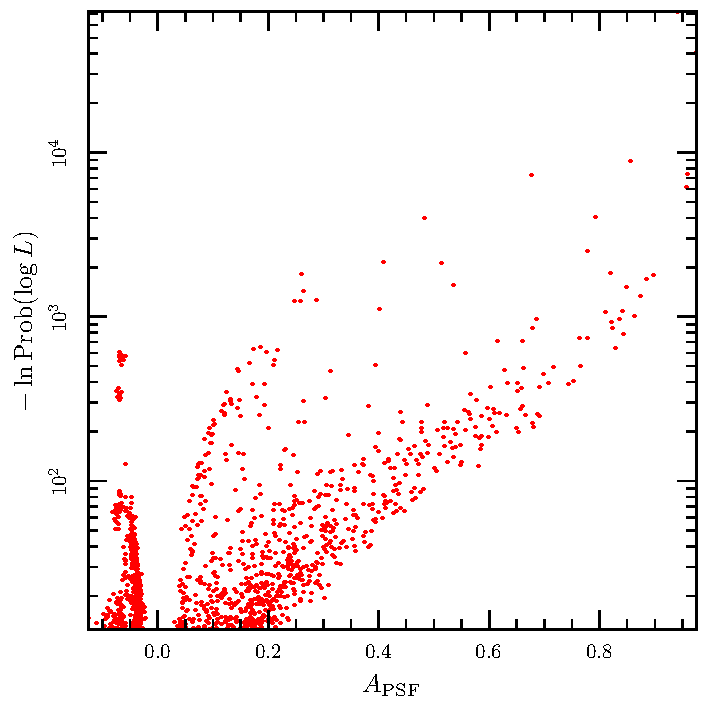
\includegraphics[width=\columnwidth]{asigcorr}
  \caption{Left: the correlation of the value $A_f$, determined from
    the means of the photon distributions, to the value of
    $A_\mathrm{PSF}$, determined from the maximum likelihood
    techinque.  Right: The values of $A_\mathrm{PSF}$ against the
    significance.}
  \label{fig:acorr}
\end{figure*}


For the sources in the preliminary catalogue ({\em i.e.} those with
$A_\mathrm{PSF}>0$ we further refine the source estimate of hte
source.  The left panel of Fig.~\ref{fig:position} depicts the change
in $\log L$ during the optimization.  Sometimes the value of $\log L$
actually decreases, but usually it increases modestly by say ten
percent.  The right panel shows the change in the position of the
source.  The size of each HEALPix region is about 0.2 degrees on a
side, so an optimization within a given HEALPix cell would result in a
typical movement of about one tenth of a degree, and the results bear
this output.  Occasionally the estmated source position moves by a
large distance indicating that the optimization has found another
nearby peak.  We use the optimized position only if the value of $\log
L$ has actually increases, and the estimated position of the source
has shifted by less than 0.5 degrees.
\begin{figure*}
  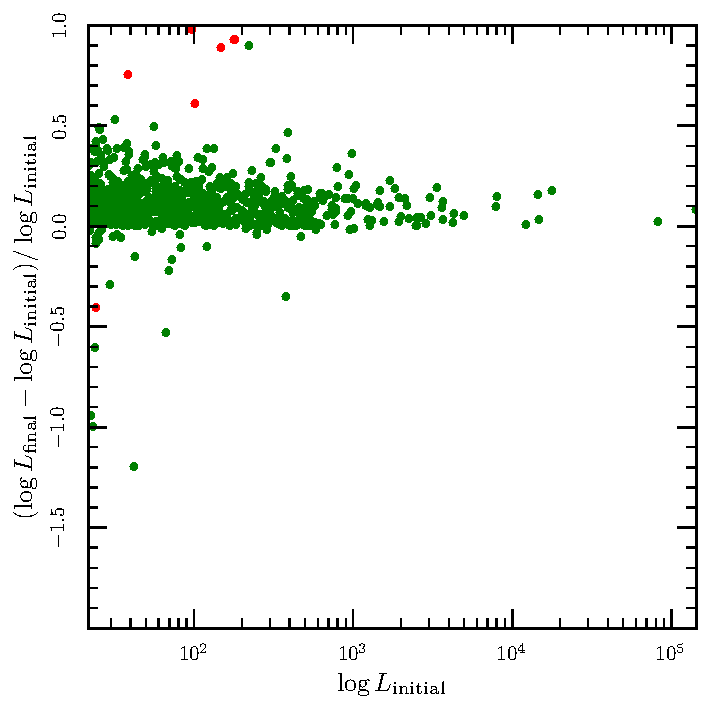
\includegraphics[width=\columnwidth]{changelogL}
  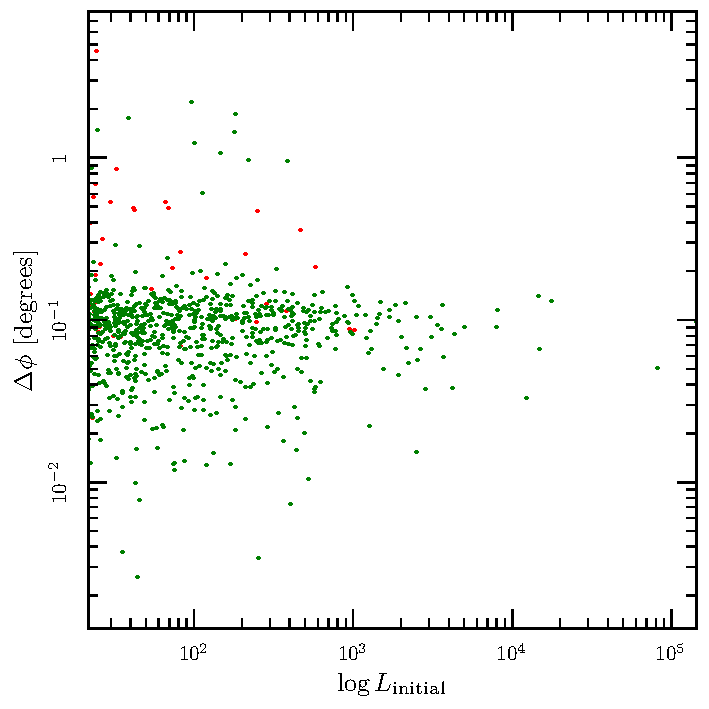
\includegraphics[width=\columnwidth]{change_position}
  \caption{Left: the relative change in $\log L$ during the position
    refinement.  Green is for sources whose positions moved less than
    one degree.  Red is for greater movement.  Right: the relative
    change in position during the position refinement.  Green is for
    sources whose positions likelihood increased.  Red is for those
    whose likelihood decreased.}
  \label{fig:position}
\end{figure*}

\section{Results}

To test the algorithm we used essentially the same data set as used to
construct the Fermi Large Area Telescope Third Source Catalog
\cite[3PSC][]{2015ApJS..218...23A}.  We used weeks 9 through 216. That
is, photons detected between 2008 August 4 (15:45:36 UTC) and 2012
July 26 (01:07:25 UTC), a span of nearly four years.  This is about
five days shorter than the span of the 3PSC observations.  We used the
good-time intervals (GTI) as defined by the Fermi team and the Pass 7
response function (\texttt{P7REP\_SOURCE\_V15}) and the Pass 7
reprocessed data.  From the form of the likelihood function,
Eq.~\ref{eq:4}, it is apparent that we do not use a model for the
background, and the key ingredient of the instrument response is the
estimate of the point-spread function \citep{2012ApJS..203....4A}.

We create two catalogues: one using photons above 1~GeV and the second
with all photons above 100~MeV.  The ten most significant sources in
the 1~GeV map are given in Tab.~\ref{tab:topten} with the refined
positions and the original detection significances.  We see a general
trend that the significances in sigma-units of the 3GFL are about
three times that of the FermiFAST technique.  The one exception in the
table is the Crab pulsar which in the Fermi analysis is split among
three sources the pulsar itself, the synchrotron and inverse Compton
components of the pulsar wind nebulae.  The FermiFAST source most
closely coincides with the pulsar, and the 3GFL significance for this
component alone is quoted in the table.
\begin{table*}
  \caption{The results for the ten most significant peaks in the 1~GeV map}
  \label{tab:topten}
  \begin{tabular}{lrrrrrrrrrrr}
    \hline
     Source & \multicolumn{1}{c}{RA} & \multicolumn{1}{c}{Dec}  & \multicolumn{1}{c}{$N_\mathrm{photons}$}  &\multicolumn{1}{c}{$\bar r^2$} & \multicolumn{1}{c}{$\bar f$} & \multicolumn{1}{c}{$S(r^2)$} & \multicolumn{1}{c}{$S(f)$} & \multicolumn{1}{c}{$A_f$}  & \multicolumn{1}{c}{$A_\mathrm{PSF}$} & \multicolumn{1}{c}{$S(\mathrm{FF})$} & \multicolumn{1}{c}{$S(\mathrm{3GFL})$} \\
    \hline

PSR J0835-4510 (Vela)     & $128.84$ & $-45.18$ & 171821 & $0.174$ & $0.521$ & $-467.5$ & $  29.5$ & $0.94$  & $0.94$ & $   378.92$ & $  1048.96$  \\ 
PSR J0633+1746 (Geminga)  & $ 98.48$ & $ 17.77$ &  90467 & $0.164$ & $0.501$ & $-349.9$ & $   0.6$ & $1.00$  & $0.97$ & $   286.73$ & $  1012.14$  \\ 
PSR J0534+2200 (Crab)     & $ 83.64$ & $ 22.02$ &  26443 & $0.204$ & $0.558$ & $-166.7$ & $  32.6$ & $0.84$  & $0.86$ & $   133.34$ & $    30.67$  \\ 
  LAT PSR J1836+5925      & $279.06$ & $ 59.43$ &  16595 & $0.167$ & $0.494$ & $-148.8$ & $  -2.5$ & $1.02$  & $0.96$ & $   121.85$ & $   438.12$  \\ 
      PSR J1709-4429      & $257.42$ & $-44.48$ &  32526 & $0.265$ & $0.614$ & $-146.9$ & $  71.3$ & $0.67$  & $0.68$ & $   121.02$ & $   360.82$  \\ 
            3C 454.3      & $343.50$ & $ 16.15$ &  14021 & $0.170$ & $0.511$ & $-135.4$ & $   4.4$ & $0.97$  & $0.96$ & $   110.98$ & $   480.74$  \\ 
  LAT PSR J0007+7303      & $  1.76$ & $ 73.05$ &  13558 & $0.224$ & $0.564$ & $-111.5$ & $  25.6$ & $0.81$  & $0.79$ & $    89.89$ & $   288.75$  \\ 
  LAT PSR J2021+4026      & $305.39$ & $ 40.45$ &  31304 & $0.331$ & $0.669$ & $-103.8$ & $ 103.9$ & $0.50$  & $0.48$ & $    89.31$ & $   237.05$  \\ 
      PSR J1057-5226      & $164.49$ & $-52.46$ &   8194 & $0.230$ & $0.570$ & $ -84.6$ & $  21.8$ & $0.80$  & $0.78$ & $    70.87$ & $   200.06$  \\ 
      PSR J2021+3651      & $305.26$ & $ 36.85$ &  22683 & $0.355$ & $0.693$ & $ -75.5$ & $ 100.5$ & $0.43$  & $0.41$ & $    65.78$ & $   145.14$  \\ 

%%   \begin{tabular}{l|rrrrrrrrrrr}
%%     \hline
%%     Source & \multicolumn{1}{c}{RA} & \multicolumn{1}{c}{Dec}  & \multicolumn{1}{c}{$N_\mathrm{photons}$}  & \multicolumn{1}{c}{$\bar r^2$} & \multicolumn{1}{c}{$\bar f$} & \multicolumn{1}{c}{$S(r^2)$} & \multicolumn{1}{c}{$S(f)$} & \multicolumn{1}{c}{$A_f$} & \multicolumn{1}{c}{$TS_\mathrm{PSF}$} & \multicolumn{1}{c}{$A_\mathrm{PSF}$} &
%%     \multicolumn{1}{c}{$\ln P(TS)$} \\
%%     \hline

%% Vela             & $128.84$ & $-45.18$ & 172081 & $0.167$ & $0.507$ & $-478.9$ & $   9.7$ & $0.98$ & $156105.48$ & $0.96$ & $-78058.94$ \\ 
%% Geminga          & $ 98.48$ & $ 17.77$ &  90450 & $0.162$ & $0.503$ & $-352.3$ & $   3.4$ & $0.99$ & $ 84019.36$ & $0.98$ & $-42015.58$ \\ 
%% Crab             & $ 83.64$ & $ 22.02$ &  26547 & $0.189$ & $0.528$ & $-175.4$ & $  15.9$ & $0.92$ & $ 21557.26$ & $0.90$ & $-10783.85$ \\ 
%% PSR J1709-4429   & $257.42$ & $-44.48$ &  33105 & $0.258$ & $0.589$ & $-152.8$ & $  56.0$ & $0.73$ & $ 17373.25$ & $0.70$ & $ -8691.73$ \\ 
%% PSR J1836+5925   & $279.06$ & $ 59.43$ &  16605 & $0.163$ & $0.491$ & $-150.3$ & $  -4.0$ & $1.03$ & $ 15372.34$ & $0.97$ & $ -7691.22$ \\ 
%% 3C 454.3	 & $343.50$ & $ 16.15$ &  14021 & $0.169$ & $0.511$ & $-135.7$ & $   4.6$ & $0.97$ & $ 12422.41$ & $0.96$ & $ -6216.15$ \\ 
%% PSR J0007.0+7303 & $  1.76$ & $ 73.05$ &  13610 & $0.212$ & $0.540$ & $-116.2$ & $  16.3$ & $0.88$ & $  9440.20$ & $0.83$ & $ -4724.90$ \\ 
%% PSR J2021.5+4026 & $305.39$ & $ 40.45$ &  30942 & $0.324$ & $0.665$ & $-107.0$ & $ 100.4$ & $0.52$ & $  8803.10$ & $0.51$ & $ -4406.32$ \\ 
%% PSR J1057-5226   & $164.49$ & $-52.46$ &   8222 & $0.227$ & $0.560$ & $ -85.8$ & $  18.9$ & $0.82$ & $  5301.47$ & $0.79$ & $ -2655.25$ \\ 
%% PSR J2021+3651	 & $305.26$ & $ 36.85$ &  22744 & $0.352$ & $0.699$ & $ -77.5$ & $ 103.8$ & $0.43$ & $  4612.93$ & $0.42$ & $ -2310.91$ \\ 
\end{tabular}
\end{table*}

\begin{figure*}
  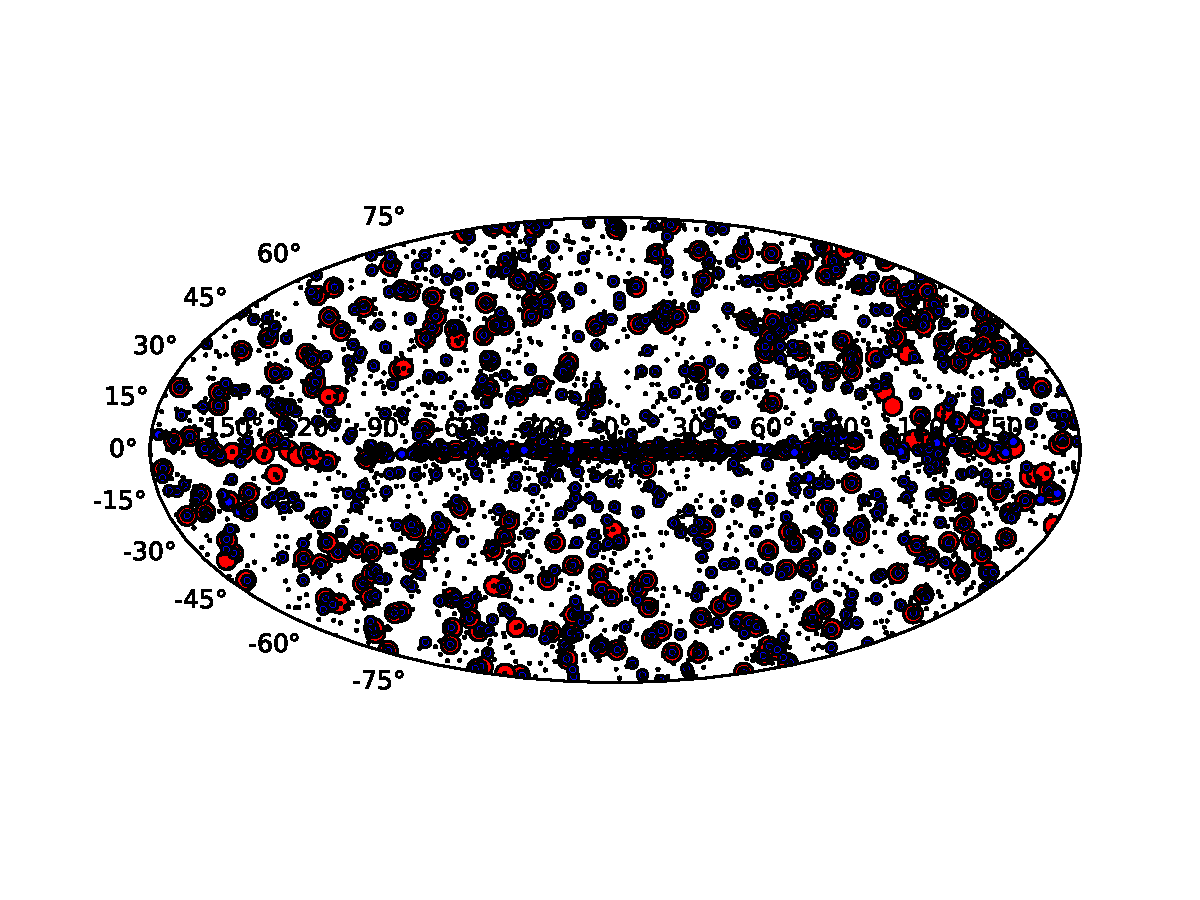
\includegraphics[width=\textwidth,clip,trim=0.6in 1in 0.8in
    1in]{source_plot}
  \caption{Sources with $\ln P(\log L)<-12.5$ (i.e. five sigma) in the
    1~GeV catalogue (small blue circles), in the 100~MeV catalogue
    (big red circles) and the 3PSC (black dots).}
  \label{fig:sources}
\end{figure*}

All of the sources detected by FermiFAST above five sigma in the 1~GeV
and the 100~MeV sample are depicted in Fig.~\ref{fig:sources}.  One
can see that nearly all of the FermiFAST sources correspond to 3PSC
sources and in fact a few may correspond to several sources.  On the
other hand, there are many 3PSC sources that do not have counterparts
in the FermiFAST catalogue.  We can examine the statistics of the
correspondances more carefully by examining the distance across the
sky between the nearest neighbours in each of the two catalogues:
FermiFAST and 3PSC.  These are plotted as the red curves in
Fig.~\ref{fig:corresponances} and the cyan curve is a multi-Rayleigh
distribution fit to the red curves.  We find that the nearest
neighbour in the 3PSC of each almost source in the FermiFAST catalogue
lies within about 1-2 arcminutes.  We must assess whether these are
chance coincidences.  If the sources in the two catalogues are not
correlated with each other ({\em i.e.} there are no real counterparts),
then one would expect that the cumulative distribution of nearest
neighbour distances to grow as a $1-\exp(\lambda \Omega)$ where
$\lambda$ is the density of sources on the sky and $\Omega$ is solid
angle enclosed by a circle centred on the object and passing through
the nearest neighbour.  Given that there are 3029 Fermi 3PSC sources
on the sky, the cumulative distribution in this case would
approximately be $1-\exp(-r^2/2\sigma^2)$ where $\sigma\approx
1.5^\circ$, so it is unlikely that these counterparts at a typical
distance of 1 arcminutes are by chance.

\begin{figure*}
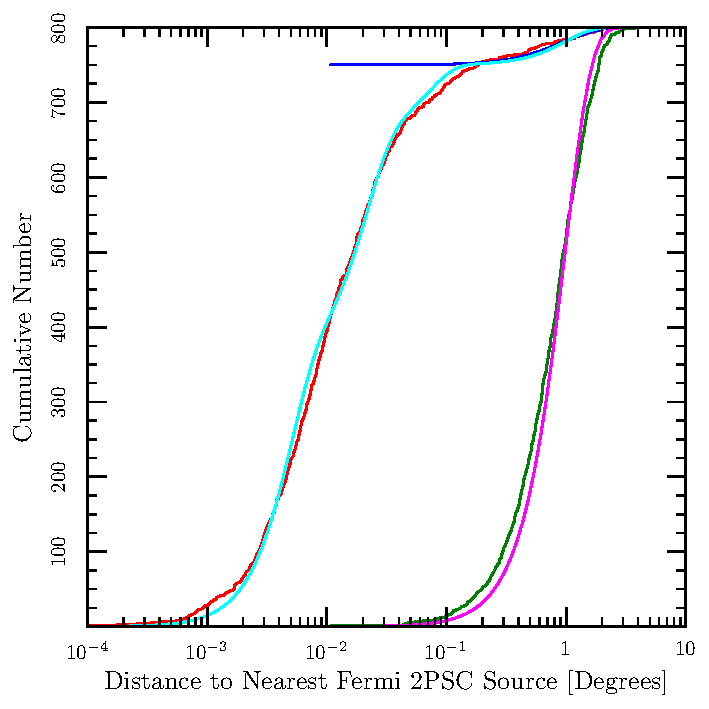
\includegraphics[width=\columnwidth]{cumff.pdf}
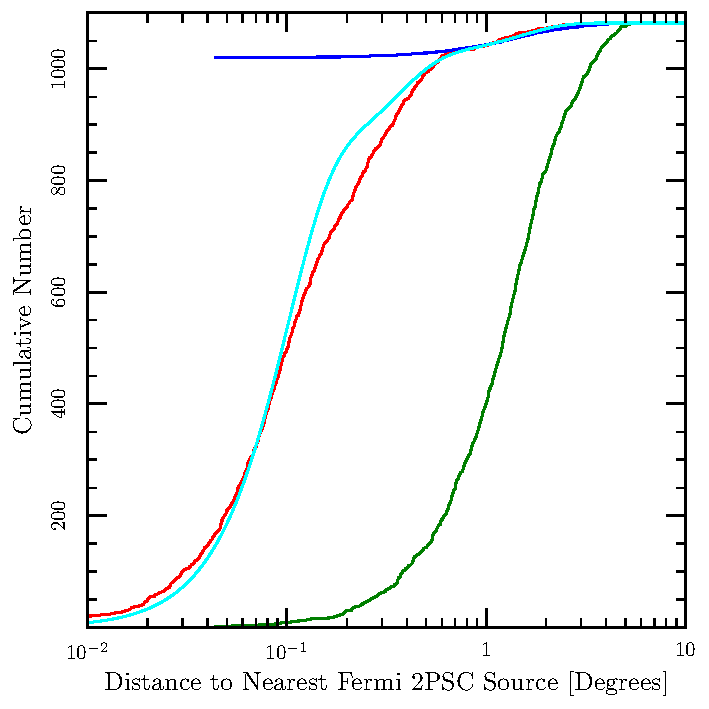
\includegraphics[width=\columnwidth]{cumff_hib.pdf}
%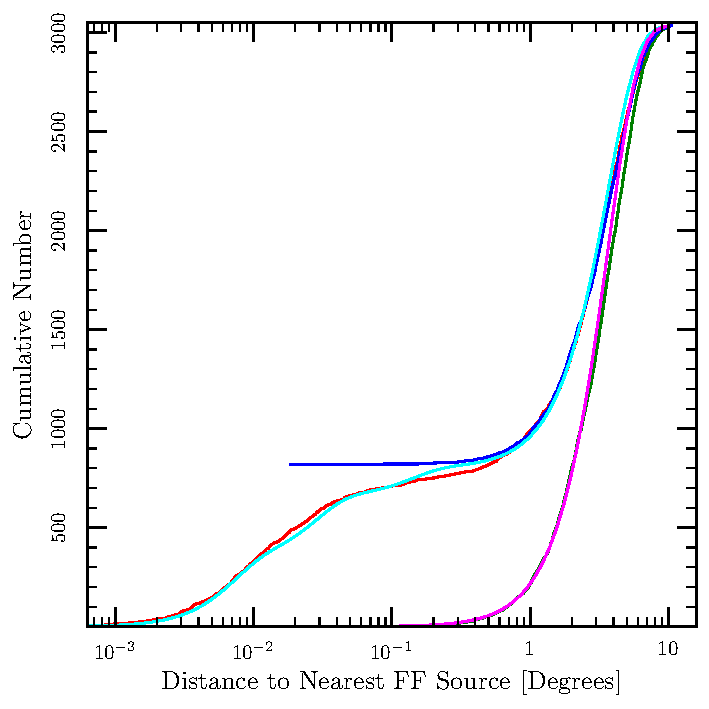
\includegraphics[width=\columnwidth]{cumfermi.pdf}
%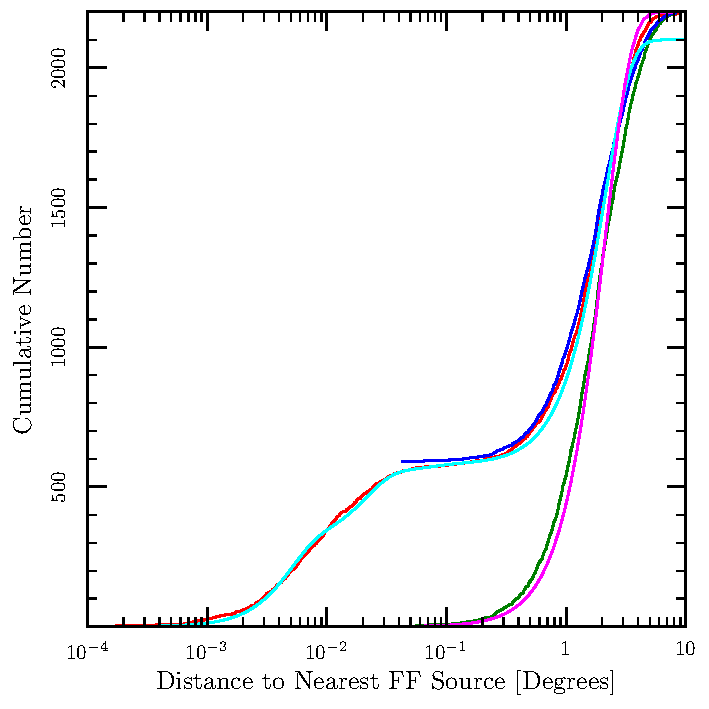
\includegraphics[width=\columnwidth]{cumfermi_hib.pdf}
\caption{The left panel give the results for all sources and the right
  panels have $|b|>10^\circ$. The distance from a Fermi FAST source to
  the nearest Fermi 3PSC source.  This demonstrates that ninety
  percent of the Fermi FAST sources are associated with sources in the
  FERMI 3PSC (across the whole sky) and nearly all at Galactic
  latitudes greater than ten degrees..  The red curve give the
  observed cumulative distribution of nearest distances.  The green
  curves give the cumulative distribution that one would expect if
  there were no associated between the Fermi FAST and Fermi 3PSC
  sources.  This is calculated by performing the same analysis as the
  red curves but with the Galactic coordinates inverted.  The blue
  curve yields the false positive rate.  The cyan and magneta curves
  are Rayleigh distributions that are fit to the observed
  distributions.  The typical positional error between associated 3PSC
  and FAST sources is 1-2~arcminutes.  }
%% \caption{The upper panels give the results for all sources and the
%%   lower panels have $|b|>10^\circ$. Left: The distance from a Fermi
%%   FAST source to the nearest Fermi 3PSC source.  This demonstrates
%%   that ninety percent of the Fermi FAST sources are associated with
%%   sources in the FERMI 3PSC.  The red curve give the observed
%%   cumulative distribution of nearest distances.  The green curves give
%%   the cumulative distribution that one would expect if there were no
%%   associated between the Fermi FAST and Fermi 3PSC sources.  This is
%%   calculated by performing the same analysis as the red curves but
%%   with the Galactic coordinates inverted.  Right: The distance from a
%%   Fermi 3PSC source to the nearest Fermi FAST source.  This
%%   demonstrates that Fermi FAST finds about one third of the Fermi 3PSC
%%   sources.  The blue curve yields the false positive rate in the case
%%   of the left panels and the completeness rate for the right panels.
%%   The cyan and magneta curves are Rayleigh distributions that are fit
%%   to the observed distributions.  The typical positional error between
%%   associated 3PSC and FAST sources is 1-2~arcminutes.  }
\label{fig:corresponances}
\end{figure*}

We also can determine the distribution of unassociated pairs from the
data itself by inverting the coordinates of the sources in one
catalogue and looking for the nearest neighbours again.  To be precise
we change the sign of the Galactic latitude and longitude of each
source in the 3PSC and repeat the nearest neighbour search.  Here all
of the correspondances will be by chance.  These results are given by
the green curves in the various panels and let us assess that nearly
all of the sources in the FermiFAST have counterparts in the 3PSC.  In
the all-sky map (left panel) in the FermiFAST, we can assess the
number of FermiFAST sources that are not in the 3PSC by fitting the
cumulative distribution with several Rayleigh distributions that
quantify the positional error for the true counterparts and the chance
of a false counterpart determined by fitting the cumulative
distribution of false counterparts with a Rayleigh distribution as
well.  We find that about 50 of the 800 sources do not have a
counterpart in 3PSC.  If we now focus on the right panel of
Fig.~\ref{fig:corresponances} we find that out of the 580
high-latitude sources in FermiFAST at most only a few lack a
counterpart in 3PSC.

One thing that is glaringly obvious from Fig.~\ref{fig:sources} is
that most sources in the 3PSC lack a counterpart in the FermiFAST
catalogue.  Both the 1~GeV and the 100~GeV version.  Given that the
algorithm outlined here is much less comprehensive that the techniques
used to generate the Fermi catalogues (there is no modelling of the
background, multiple sources or spectra), this is not surprising.
However, it is useful to figure out what sources are missing from the
FermiFAST catalogue and why.  Fig.~\ref{fig:fermi_comp} 
shows the relationship between the significances of a source
assigned by FermiFAST and by the 3PSC.  In particular the 3PSC
significances are three times larger (the upper line) than FermiFAST
typically, so if both apply a threshold of five sigma, FermiFAST will
find fewer sources.  However, there is a large population of sources
for which the two likelihoods are similar or the FermiFAST likelihood
is larger.  Since FermiFAST does not perform any spectral modelling,
perhaps these sources have poor spectral fits in the 3PSC, yielding
smaller likelihoods.  Furthermore, this indicates a discovery space
for FermiFAST to find point sources where we do not have a good prior
notion of the spectral model.  The outlying point in the lower-right
is the Crab pulsar whose 3PSC likelihood is artificially too low due
to the way it is fit within the catalogue.

To understand further whether FermiFAST is simply missing less
significant 3PSC sources we can look at the cumulative distribution of
3PSC significances of sources that appear in the FermiFAST 1~GeV
catalogue and all of the 3PSC sources in Fig.~\ref{fig:sign-dist}.  We
see that FermiFAST catalogue is essentially complete for all 3PSC
sources above about 18-sigma, so FermiFAST can quickly (in six minutes)
generate a sample from the Fermi data stream of the upper quartile of
sources that would appear a Fermi catalogue using the full likelihood
technique to construct the catalogue.
\begin{figure}
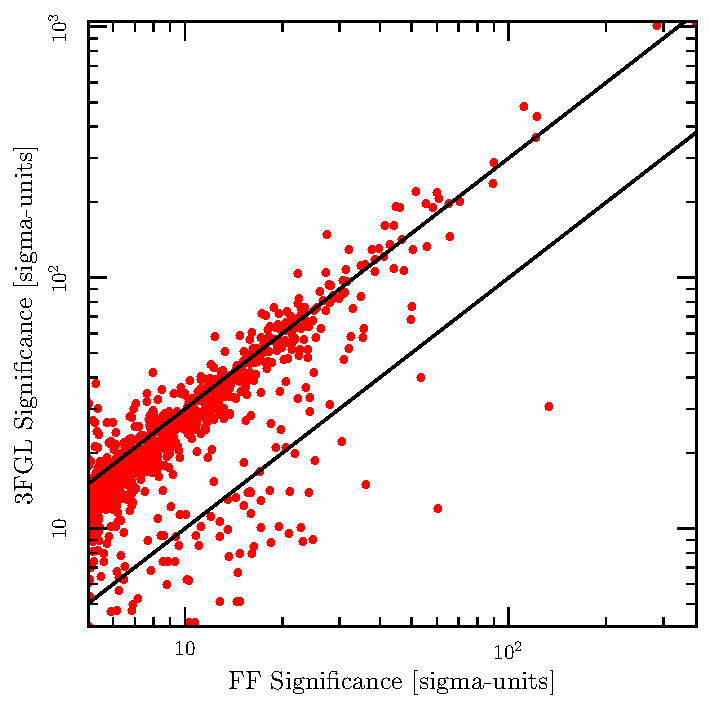
\includegraphics[width=\columnwidth]{sign-comp}
\caption{3PSC Significances vs Fermi FAST.  The red points are
  where the counterparts lie within $0.2^\circ$ of each other, the
  green the counterparts lies between $0.2^\circ$ and $1^\circ$, and
  the blue have counterparts further than $1^\circ$ away. }
\label{fig:fermi_comp}
\end{figure}

\begin{figure}
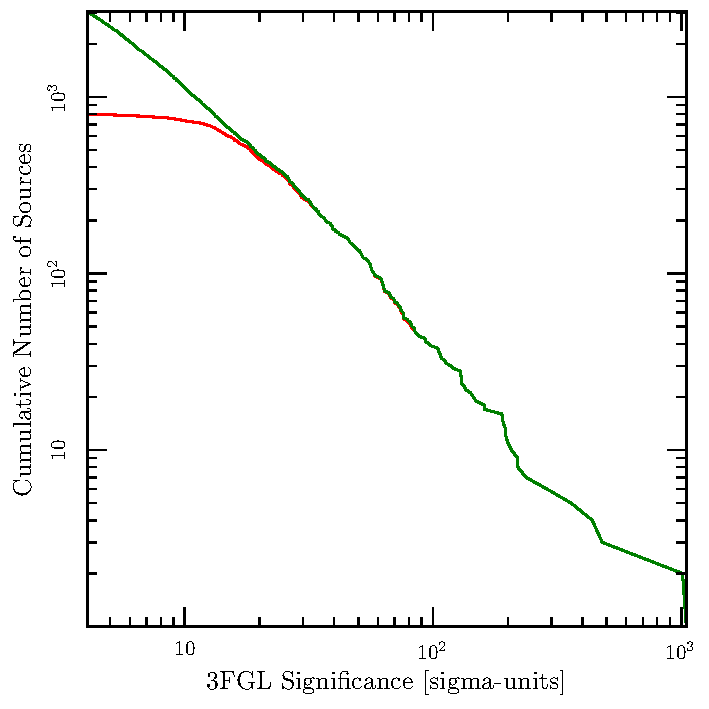
\includegraphics[width=\columnwidth]{sign-dist}
\caption{
  Cumulative distribution of 3PSC significances for the entire 3PSC
  (blue) and the entire Fermi FAST 1-GeV catalogue with a five-sigma
  cut (green) and Fermi FAST where the 3PSC counterpart lies within
  $0.2^\circ$ (red) again with a five-sigma cut.  The blue and cyan
  give the same as green and red but with a three-sigma cut.}
\label{fig:sign-dist}
\end{figure}

The question arises: is it possible to do better? We can reduce the
significant threshold for find sources in the 1-GeV FermiFAST
catalogue.  We expect that the number of sources that do not have firm
associations in the 3PSC to increase but also for the completeness to
increase as well.  We can use the empirical distance distribution for
the false matches depicted in yellow in Fig.~\ref{fig:ffl_comp} to
split the distribution of the matches between Fermi FAST and the 3PSC
statistcally into the true matches and the false matches to measure
the completeness and purity of the samples.  The contribution of the
false matches to the cumulative distributions is depicted in the same
colour as the measured distributions but dashed.  The distribution of
the close matches here is somewhat different than in
Fig.~\ref{fig:corresponances} because we have not used the improved
localizations to find the matches.  The localization improvement tends
to fail more often for sources of low significance (see
Fig.~\ref{fig:position}).  Tab.~\ref{tab:comppure} gives the results
of this trial.  The key result is that the five-sigma sample is very
pure; only about five percent of the sources lack firm associations in
the 3PSC.  On the other hand, if one is willing to sacrifice the
purity of the sample, one can achieve nearly 50\% completeness
relative to the 3PSC by reducing the significance threshold to
$3-\sigma$.  Fig.~\ref{fig:sign-dist} shows by accepting a lower
purity one can get a complete 3PSC sample about about ten-sigma,
comprising nearly half of the 3PSC sample.
\begin{table}
  \caption{Completeness and Purity}
  \label{tab:comppure}
  \begin{tabular}{l|rrrrr}
    \hline
    Threshold & \multicolumn{1}{c}{Sources} & \multicolumn{1}{c}{True} & \multicolumn{1}{c}{False} & \multicolumn{1}{c}{Purity} & \multicolumn{1}{c}{Comp} \\
    \hline
    $3-\sigma$   & 1727 & 1400 & 327 & 81.1\% & 46\% \\
    $3.5-\sigma$ & 1312 & 1180 & 132 & 89.9\% & 39\% \\
    $4-\sigma$   & 1076 &  995 &  81 & 92.5\% & 33\% \\
    $4.5-\sigma$ &  923 &  865 &  58 & 93.7\% & 29\% \\
    $5-\sigma$   &  800 &  755 &  45 & 94.3\% & 25\%  
  \end{tabular}
\end{table}

\begin{figure}
  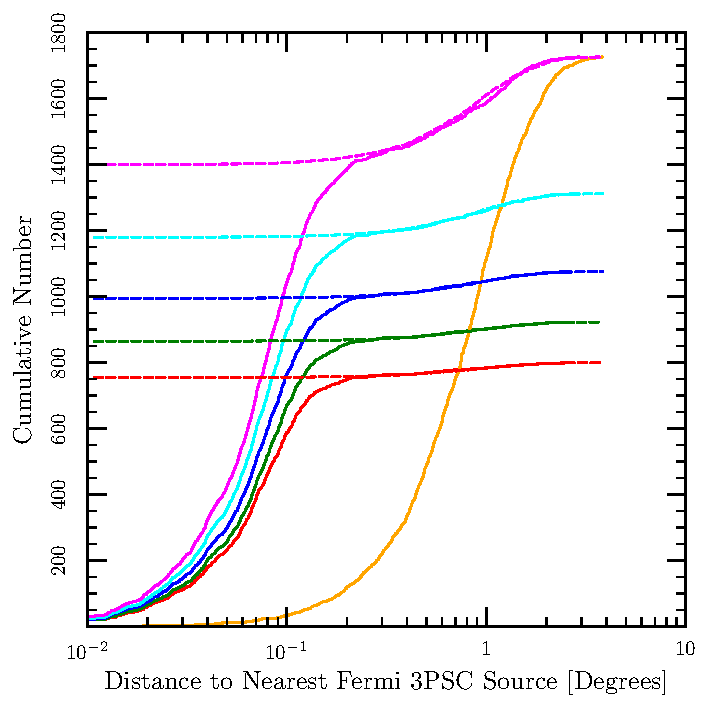
\includegraphics[width=\columnwidth]{cumfflo_comp}
  \caption{The cumulative distribution of distances between sources in
    Fermi FAST and 3PSC for various significance thresholds from top
    to bottom of 3-sigma, 3.5-sigma, 4-sigma, 4.5-sigma and 5-sigma.
    The dashed curves that start above zero and join each cumulative
    distribution at large radii trace the cumulative distribution of
    distances for the false matches in each sample.}
  \label{fig:ffl_comp}
\end{figure}

We saw in Fig.~\ref{fig:fermi_comp} that in general the FermiFAST
significances and the 3PSC significances are well correlated with
However, for about one fifth of the sources $S(\mathrm{3PSC}) < 2 S(\mathrm{FF})$
and for about one tenth $S(\mathrm{3PSC}) < S(\mathrm{FF})$.
This demonstrates that at least for a fraction of
the 3PSC the FermiFAST technique is more sensitive, so the sources
that do lie in the FermiFAST catalogue but not the 3PSC may just be a
class of sources to which the 3PSC is less sensitive, perhaps sources
for which the suite of spectral models employed in the construction of
the 3PSC to do apply.  On the other hand, these unassociated sources
could simply be regions where the diffuse background is especially
bright and clumpy.  Because the FermiFAST technique assumes that the
background is smooth on the scale of the PSF, it would find a source
where the background is locally strong.  We possibly see the opposite
of this effect in Fig.~\ref{fig:acorr} where FermiFAST finds negative
sources that are most likely places where the background is locally
weak.

{\bf talk about the 100~MeV catalogue }

\section{Discussion}

We have outlined a technique that can rapidly find point sources from
the photon data from the Fermi telescope.  If one focusses on the
photons above 1~GeV, one can reproduce about half of the 3PSC using
the 3PSC data set in about six minutes with a false association rate of
less than twenty percent.  There are several immediate applications of
this technique that come to mind as well as several avenues of
potential improvements to increase the sensitivity and specificity
and the data that we learn about each source.  First, we will discuss
some potential applications.

The speed of the technique opens several possible exploratory research
paths.  One can search fractions of the data stream for potential
sources that we active for a portion of the complete 3PSC observation
time and so did not reach the threshold for detectability over the
entire observation but were sufficiently bright to be detected over a
shorter window.  Given the large variability of blazars which form the
bulk of the sources outside the plane of the Galaxy, this is an
interesting avenue.  In fact although the 3PSC catalogue contains many
more sources than the 2PSC, many sources are absent in the 3PSC that
were in the 2PSC.  Some of these may have been spurious, but others
could have simply been variable, so the search for variable sources
provides an exciting avenue.  Furthermore, the sources in the
FermiFAST catalogue that are not in the 3PSC would be great seeds for
a full characterization using the Fermi tools.  Are these potential
sources simply knots in the gamma-ray background or do they remain
significant even with the full analysis?


A second important direction is to use the FermiFAST algorithm to
generate a catalogue of sources, most likely not as deep as the 3PSC
and then use the catalogue for further statistical analysis of the
various populations.  Now what are the advantages of this when one
considers that the 3PSC already exists?  Because the FermiFAST
catalogue only requires a few minutes to generate one can explore the
statistical biases, selection and uncertainities in the catalogue
through simulated data much more easily than for the full 3PSC
catalogue.  A first step would be to insert artificial sources of
known fluxes and spectra into the data stream.  This could be down in
parallel by again inserting the sources on a HEALPix grid so that the
regions of interest for each source (Fig.~\ref{fig:expmap}) do not
overlap over the energy range considered.  Now we can measure the
relationship between the flux and significance throughout the sky to
obtain the selection function for the survey.  This is crucial
ingredient to determine the luminosity function of the underlying
population.  Because the underlying sources may be variable, we could
also insert variable sources into the data stream as well and combine
this with the time slicing analysis described in the previous
paragraph and develop for example a catalogue of blazars as a function
of mean luminosity and variability that is both statistically well
characterized and possibly contains new objects that were not
discovered in the previous Fermi catalogues.  Of course, many of the sources
will have already been detected by Fermi and possibly followed up
with further measurements, the key element here would be that the sample
would be statistically well characterized, so clear conclusions about the
population could be obtained.

Using the existing data stream without inserting sources, one could
characterize whether the measurement significances of the individual
sources are reasonable and whether the variability measurement
determined say in an analysis as outlined earlier is significant.  The
first step would be to resample the photon data stream through a
bootstrap --- this would generate a new list of photons by selecting
the same number of photons from the original list but with
replacement, so that the same photon could appear many times in the
new sample and of course some photons won't appear at all.  Each new
list of photons would generate new catalogue to determine what
properties of the sources and the catalogue as a whole are robust
against the Poisson fluctuations in the data stream.  This would
verify the underlying assumptions of the significances of the sources
as well as determine how sources near the detection threshold enter
and leave the sample.  Because the sample is dominated by the faintest
sources near the detection threshold (see Fig.~\ref{fig:fermi_comp}),
understanding this effect is again crucial to understand the sample.

To detect point sources from the Fermi photon data stream, we only
used the data stream and the estimates of the point-spread
function. There is additional data available that could help to
improve the sensitivity of the technique, reduce the number of false
positives and better characterize the sources detected.  First, the
likelihood function, Eq.~\ref{eq:4}, assumes that the gamma-ray
background is smooth everywhere.  However, we know from independent
measurements, for example the Galactic synchrotron emission, that the
gamma-ray background is likely to be clumpy and the Fermi team
provides estimates of this background \citep[e.g.][]{Fermi1602.07246}.
By combining this background
estimate along with the integral of the effective area and time that a
particular direction and energy was observed, we can develop an
improved likelihood function that includes the estimated background.
This could reduce both the number of candidate sources detected with
$A_\mathrm{PSF}<0$ and the number of candidate sources without
counterparts in the 3PSC.  The addition of this information would not
dramatically increase the time to construct the catalogue (we have
already included this functionality in the software but it is not yet
well characterized).

One could also take an alternative route.  Looking again at
Eq.~\ref{eq:4}, we can use the relative size of the two terms in the
brackets to assign a fraction of each photon to the source and to the
background.  Again if we include information on the effective area and
the exposure time, we obtain an estimate of the spectrum from each
source and from the background.  Because a given photon could be
assigned to several sources as well as the background, we would also
have to develop a good statistical model to split the photon among the
sources.  Of course, a first estimate could be obtained by ignoring
the fact that several potential sources could claim a given photon and
resolve the gamma-ray data into sources and background \citep[as done
  by][]{2015A&A...581A.126S}. This would provide an independent
confirmation of the structure of the gamma-ray background, but perhaps
more importantly it would yield an estimate of the spectrum of each
source. One could include a fit to the source spectrum as in the
standard Fermi analysis either in the initial likelihood calculation
or after the sources have been detected.  In the first case this might
improve both the sensitivity as we could find fainter sources against
the background if they follow one of the spectral models and the
specificity by excluding potential sources that do not follow the
models.

FermiFAST provides the infrastructure both for exploratory analysis of
the Fermi data to find new sources and new variable sources and also
to create a sample of sources for population studies that can be
characterized comprehensively by Monte Carlo simulation of the
detection technique.  The latter may allow new understanding of the
population of Galactic and extragalactic gamma-ray sources and their
evolution.

\section*{Acknowledgments}

Jeremy Heyl would like to thank Elisa Antolini for the conversations
that formed the impetus for this paper.  The software used in this
paper and the catalogues generated are available at
\url{http://ubc-astrophysics.github.io}.  We used the VizieR Service,
the NASA ADS service, the Fermi Science Support Center, the
astrometry.net $k-d$~tree library, the HEALPix and HEALPy libraries
and arXiv.org. This work was supported by the Natural Sciences and
Engineering Research Council of Canada, the Canadian Foundation for
Innovation, the British Columbia Knowledge Development Fund and the
Bertha and Louis Weinstein Research Fund at the University of British
Columbia.

\bibliography{fermi}
\bibliographystyle{mn2e}


\label{lastpage}

\end{document}

